\documentclass{extarticle}
\usepackage{setspace}
\usepackage{graphicx}
\usepackage{cite}
\usepackage{fontenc}
\usepackage{helvet}
\usepackage[utf8]{inputenc}
\usepackage{times}
\usepackage{url}
\usepackage[paper=a4paper,left=17.5mm,right=17.5mm,top=35.8mm,bottom=35.8mm]{geometry}
\usepackage{titlesec}
\setlength{\columnsep}{0.8cm}

\titleformat*{\section}{\large\bfseries}
\titleformat*{\subsection}{\bfseries}

\begin{document}
	
	\twocolumn[
	\begin{@twocolumnfalse}
	
	\begin{center}
		\Large\textbf{Musikdownloads - Geschichtliches, Formate, Geschäftsmodelle} \\~\\
		\large Martin Baumgartner, Daniel Krall \\~\\
	\end{center}
	\thispagestyle{empty}
	\end{@twocolumnfalse}]
	
		\singlespacing
		\begin{center}
			\large\textbf{Abstract}	\\
		\end{center}
		\textit{Von den ersten Tonaufzeichnungen bis zu modernen Streamingdiensten hat die Musikbranche große Fortschritte gemacht. Im folgenden Paper wird zuerst auf die Geschichte der Tonaufzeichnung eingegangen, dann auf verschiedene verlustfreie und verlustbehaftete Audioformate und deren Funktion und zum Schluss werden die verschiedenen Geschäftsmodelle aufgezeigt.} \\~\\
		
		\section{Geschichtliches}
		\subsection{1800}
		Anfang des 19ten Jahrhunderts entdeckte der französische Mathematiker und Physiker Jean Marie Constant Duhamel, dass man eine Stimmgabel mit einem Bleistift kombinieren konnte, so dass auf Papier die Vibrationen der Stimmgabel als Wellenlinie wiedergegeben werden konnten. Der englische Physiker Thomas Young baute daraufhin den ersten Kymographen, mit dem die Vibrationen auf einer rotierenden Walze aufgezeichnet werden konnten. Das Prinzip seiner Entwicklung bildet bis heute die Basis für die Aufzeichnung und Analyse von Tönen. \cite{Disc1}
		
		\subsection{1860}
		Aus dem Jahr 1860 stammt die erste Tonaufnahme, das Kinderlied "Au clair de la lune", welches 2008 rekonstruiert werden konnte. Der französische Drucker und Korrekturleser Edouard-Léon Scott de Martinville meldete im März 1857 seinen Phonautographen als Patent an, mit diesem Apparat wurde die Tonaufnahme aus dem Jahr 1860 über eine an einer Membran angebrachten Schweineborste auf einer russgeschwärzte, rotierenden Walze aufgezeichnet. Scott der Martinville dachte allerdings nicht daran, mit seinem Phonautograph die Aufzeichnungen auch wiederzugeben. Dies gelang erst 1878 mit dem Phonograph des US-Amerikaners Thomas Alva Edison. \cite{Disc2}
		
		\subsection{1890}
		Im Jahr 1898 patentierte der dänische Erfinder Valdemar Poulsen das Telegraphon. Es handelte sich dabei um den ersten Apparat zur Tonaufzeichnung mittels elektromagnetischer Induktion. Ein Klaviersaitendraht aus Stahl, der auf eine Walze aufgewickelt war, diente dabei als Trägermedium. Verbesserte Versionen des Apparats konnten Gespräche von bis zu 30 Minuten Länge aufzeichnen. Aufgrund der mäßigen Aufnahmequalität  und der geringen Lautstärke hielt sich die Nachfrage in Grenzen. Erst 20 Jahre später wurde die Idee wieder aufgegriffen, da zu diesem Zeitpunkt Audioverstärker verfügbar waren. \cite{Disc3}
		
		\subsection{1920}
		Ende der 1920er Jahre enstanden die ersten Tonbandgeräte, somit war es erstmals möglich, Geräte an Empfänger anzuschließen, um so Programme aus dem immer stärker verbreiteten Rundfunk mitzuschneiden. \cite{Reininger1928}
		
		\subsection{1960}
		Im Jahr 1963 wurde auf der Berliner Funkausstellung von Philips die Kompaktkassette (Compat Cassette, kurz CC) vorgestellt. Bei dieser Erfindung wurden zwei magnetisierte Tonbänder nebeneinander angeordnet und in ein Kunststoffgehäuse eingebaut. Eine Kassette ist wendbar, kann also beidseitig bespielt werden. Auf der Austellung wurde auch der erste dazugehörige Kassettenrekorder, der Philips EL3300 vorgestellt. In den 1970er Jahren hatte sich die Kompaktkassette längst durchgesetzt, Ende der 70er Jahre wurde dann der erste Walkman vorgestellt, ein kompakter, tragbarer Kassettenrekorder. \cite{Disc4}
		
		\subsection{Ab 1980}
		Ab 1982 begann mit der Einführung der Compact Disc (CD) von Philips und Sony die Digitalisierung der Musik. Die meisten anderen Hersteller von CDs hatten ihre Produkte lizenziert, wodurch das Produkt schnell standardisiert wurde, außerdem verteilte Philips Informationen über die Herstellung von CDs, wodurch dies auch bei den meisten Herstellern einheitlich geschah. \cite{CDeins} \\
		Im Vergleich zum Plattenspieler wird die CD nicht berührt und dadurch zerkratzt, sondern mit einem Laser abgetastet. Musik muss, bevor sie auf eine CD gespielt werden kann, digitalisiert werden, dies geschieht mittels Pulscode-Modulation (PCM). In den 2010er Jahren musste die CD nach und nach digitalen Medien wie MP3 weichen. Im Jahr 2017 lag der Umsatz durch CD- und LP-Verkäufe jedoch immer noch bei 53\% des Gesamtumsatzes. \cite{CDzwei}
		
		\section{Formate}
		\subsection{Puls-Code-Modulation (PCM)}
		Mit der PCM wird ein analoges Audiosignal digitalisiert. Dabei wird ein Signal mit einer konstanten Abtastrate (also in regelmäßigen Zeitabständen) abgetastet. Diese Abtastrate wird in Hertz oder Zyklen pro Sekunden angegeben. Die einzelnen Abtastungen werden dann binär codiert. \cite{PCMtext} \\
		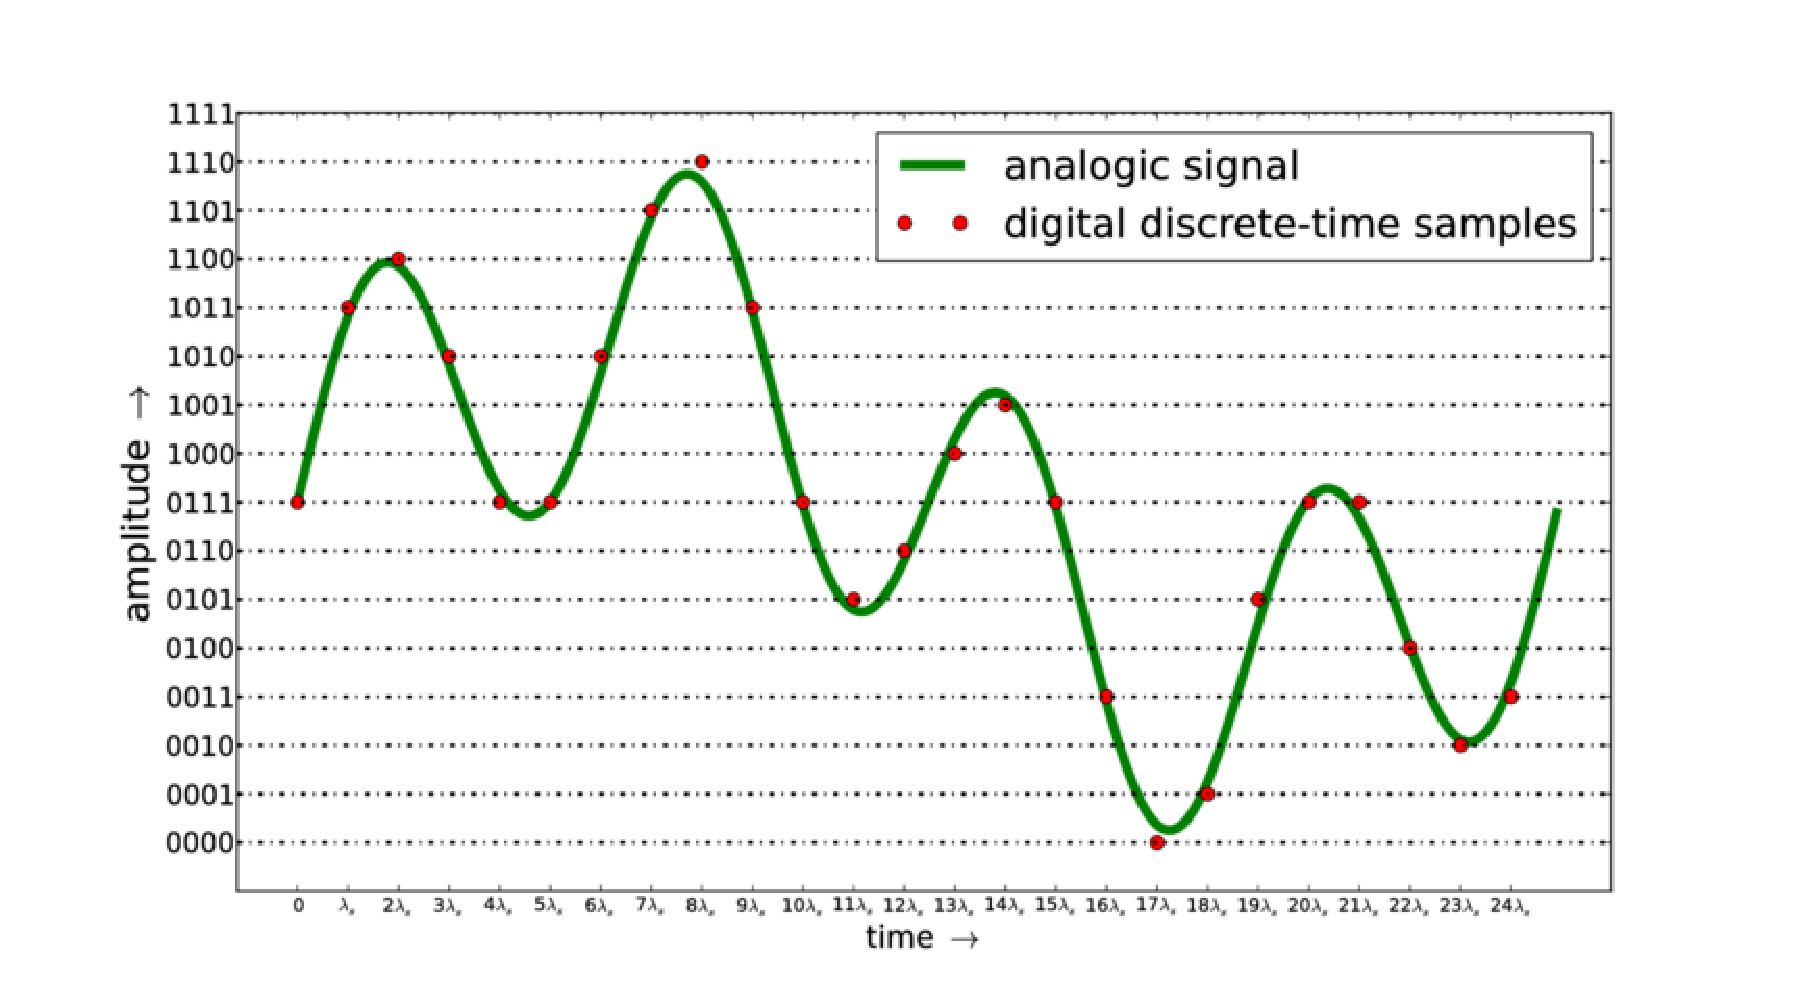
\includegraphics[width=\columnwidth]{PulsCodeMod.eps}
		\begin{center} Abtastungen in Rot dargestellt \cite{PCMimg} \end{center}
		
		\subsection{WAVE (Verlustfrei)}
		WAVE (bzw. WAV) ist ein verlustfreies Audioformat, entwickelt von Microsoft \& IBM. Im Vergleich zu verlustbehafteten Formaten, ist die Audioqualität höher, im Gegenzug sind die Dateien jedoch auch um einiges größer. WAVE setzt auf dem Resource Interchange File Format (RIFF), einem Containerformat, auf. Die Signale werden in Pulse-Code-Modulation codiert und in Chunks gespeichert. Dabei können Dateien mit 8- bzw. 16-Bit-Samples mit einer Abtastrate von 11.25Hz und 44.100Hz aufgenommen werden. \cite{WAVE}
		
		\subsection{AIFF (Verlustfrei)}
		Das Audio Interchange File Format wurde von Apple entwickelt und ist das Gegenstück zu Microsofts WAVE-Format. Es wurde Ende der 1980er Jahre als Standard Audio-Format für Macintosh Rechner entwickelt. Das Format basiert auf dem Interchange File Format von Electronic Arts (EA). \cite{AIFF1} \cite{AIFF2}
		
		\subsection{FLAC (Verlustfrei)}
		Der Free Lossless Audio Codec ist ein von der Xiph.org Foundation entwickelter Audio-Codec. Das Format ist verlustfrei, trotzdem werden die Daten bei diesem Codec komprimiert. Das Format ist frei verfügbar, die Nutzung ist also nicht durch Patente beschränkt. Digital Rights Management (DRM), also einen Kopierschutz unterstützt Format nicht. \cite{FLAC} \\
		Bei der Kompression werden die Daten zuerst in Blöcke zu 1000-6000 Samples geteilt, dann wird Stereo (Links-Rechts) in Mitte-Seite gewandelt, da Links und Rechts meist sehr ähnlich sind. Durch Linear Predictive Coding (LPC) werden zukünftige Werte anhand vorheriger Werte vorhergesagt, so nähert man sich dem Werteverlauf eines Blocks an. Ein Fehlersignal, welches den Unterschied zwischen tatsächlichem und modelliertem Signal enthält wird zusätzlich übertragen. \\
		FLAC erlangte 2004 große Bekanntheit, als die Band Metallica bekanntgab, ihre Konzertmittschnitte nur noch in diesem Format anzubieten. \cite{FLACWiki}
		
		\subsection{ALAC (Verlustfrei)}
		Der Apple Lossless Audio Codec ist ein Open-Source Format, welcher von Apple im Jahr 2011 freigegeben wurde. Der Codec ist FLAC sehr ähnlich, jedoch kann ALAC auch in iTunes und auf iOS-Geräten verwendet werden, weshalb das Format in Musikstudios weit verbreitet ist. \cite{ALAC}
		
		\subsection{MP3 (Verlustbehaftet)}
		MP3 ist der am weitesten verbreitete Audio-Codec der Welt. \cite{mp3} \\
		Das bekannte Format wurde 1982 vom Frauenhofer-Institut entwickelt. Mit diesem Format fand der Musikdownload über das Internet Aufschwung, da die kleinen Datein leicht verbreitet werden konnten. Das Prinzip der Kompression ist, Teile des Audiosignals, die für das menschliche Gehör nicht wahrnehmbar sind, zu entfernen, wodurch Informationen entfernt und somit auch die Dateigröße verringert wird. Für die meisten Menschen ist ab einer Datenrate von 200kbps kein Unterschied zum originalen, unkomprimierten Signal feststellbar. \cite{mp3aac} \\
		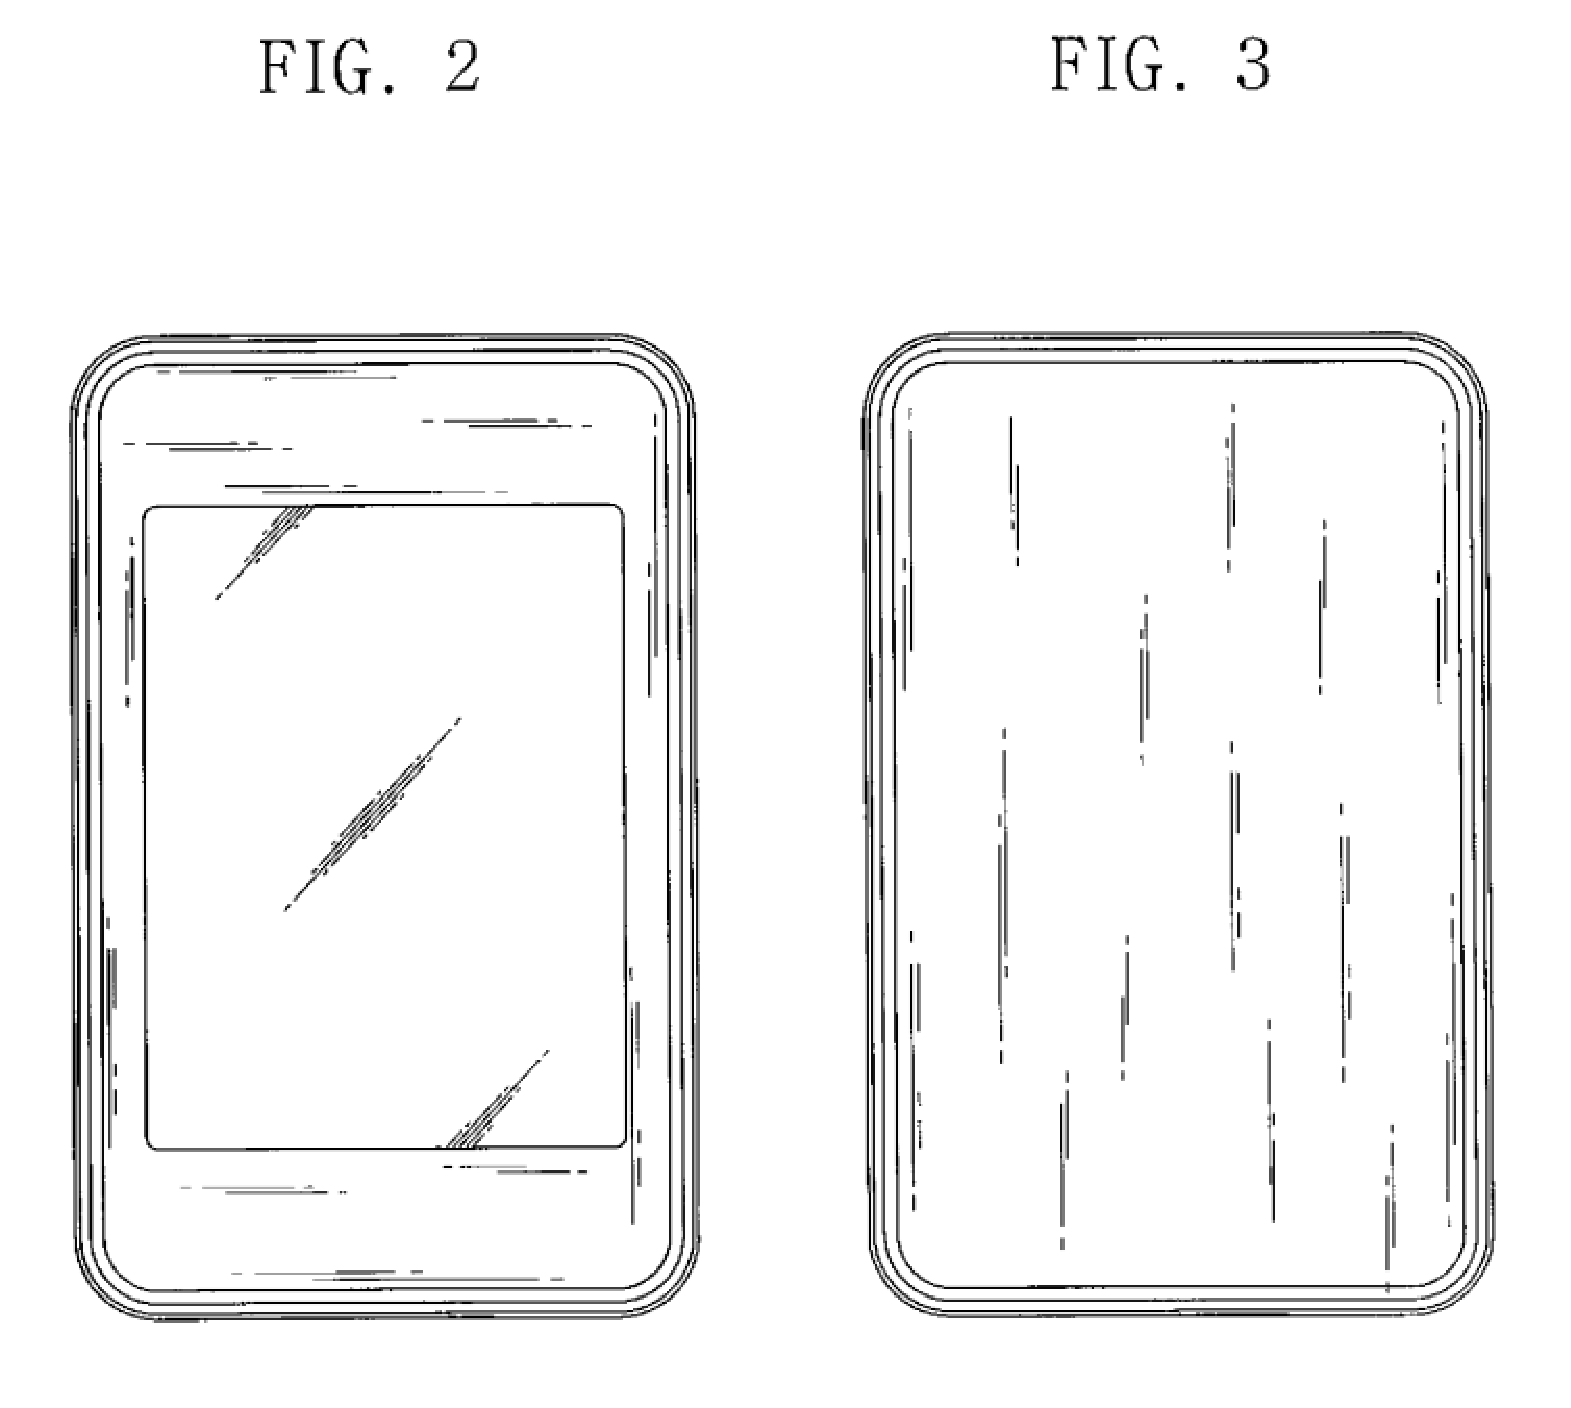
\includegraphics[width=\columnwidth]{patent.eps} \\
		\begin{center} Patent eines MP3-Players von LG Electronics \cite{patent} \end{center}
		
		\subsection{AAC (Verlustbehaftet)}
		Mit dem Advanced Audio Coding Format wurde der Nachfolger vom MP3-Format veröffentlicht. Durch Verbesserungen werden hier eine besser Audioqualität und geringere Datengrößen erreicht. Ablösen konnte AAC das MP3-Format bisher jedoch nicht. \cite{mp3aac}
		
		\subsection{Ogg Vorbis (Verlustbehaftet)}
		Ogg Vorbis ist ein verlustbehafteter Codec von der Xiph.org Foundation. Genau wie FLAC ist auch Vorbis lizenzfrei und nicht durch Patente beschränkt. Die Kompression ist der von MP3 ähnlich, jedoch effizienter. Aufgrund seiner Streamingfähigkeit findet Vorbis weite Verbreitung. \cite{vorbis}
		
		\section{Geschäftsmodelle}
		\subsection{Digital Rights Management (DRM)}
		Mit DRM, also der digitalen Rechteverwaltung, wird es Urhebern möglich gemacht, den Zugriff auf Inhalte/Dateien zu schützen, da digitale Inhalte leicht zu kopieren und zu \\ vervielfältigen sind. Dafür müssen die Zugriffe kontrolliert werden, sodass nur berechtigte Nutzer auf die Inhalte zugreifen können, außerdem muss sichergestellt werden, dass Daten nicht verändert werden können. Umgesetzt wird dies meist mit einer Software des Anbieters, welche den Inhalt verschlüsselt und können nur durch abgespeicherte Rechte eines Nutzers entschlüsselt werden. \\ 
		DRM findet jedoch auch Widerstand bei den Nutzern, vor Allem, wenn die Nutzung auf nur ein Gerät beschränkt ist, oder bei fehlerhaften Schutzvorrichtungen. \cite{drm} \cite{drmReport} \\
		Beispiele für DRM-Systeme wären Apple Fairplay, Windows Media DRM, Open Mobile Alliance DRM und Marlin DRM. \cite{drmsysteme} \\
		\\ \begin{center}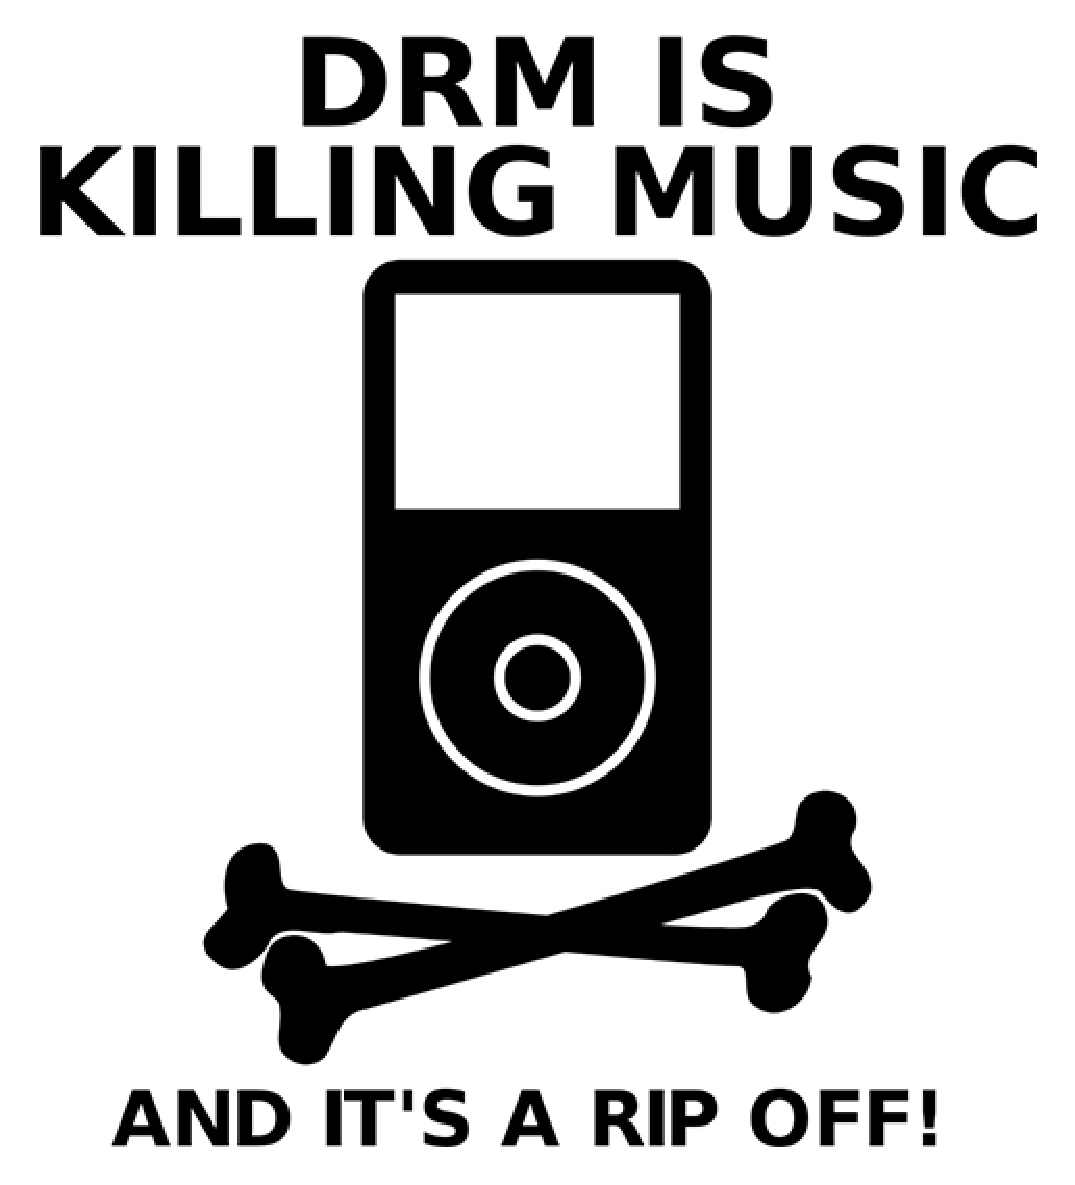
\includegraphics[width=5cm]{DRM.eps} \cite{drmKritik}\end{center}
		
		\subsection{À la carte}
		Hierbei handelt es sich um das Standard-Geschäftsmodell, auch als Download-to-Own bezeichnet, das heißt, ein Song oder Album wird gekauft und das gekaufte Produkt kann dann heruntergeladen werden. Die Nutzung des Produkts wird, wenn vorhanden, durch eine DRM-Lizenz beschränkt. \cite{modelleWiki}
		
		\subsection{Abonnement}
		Gegen eine monatliche Bezahlung kann beim Abonnement eine bestimmte Anzahl an Titeln heruntergeladen werden. Die Nutzung wird wieder durch die DRM-Lizenz beschränkt. \cite{modelleWiki}
		
		\subsection{Flatrate}
		Bei einer Flatrate wird monatlicher ein bestimmter Betrag bezahlt, durch den man auf eine Datenbank Zugriff erhält, von der eine beliebige Anzahl an Songs heruntergeladen werden kann. Durch DRM-Lizenzen ist die Nutzung teilweise jedoch stark beschränkt, so besteht die Möglichkeit, dass die gedownloadeten Titel nach Ablauf der Flatrate nicht mehr abgespielt werden können. Außerdem ist das Brennen auf CDs meist verboten. \cite{modelleWiki}
		
		\subsection{Streaming}
		Auch beim Musikstreaming fällt eine monatliche Gebühr an, im Vergleich zur Flatrate werden die Titel jedoch nicht heruntergeladen, sondern online abgespielt. Auch hier hat der Nutzer auf alle Titel der Datenbank Zugriff und kann sich eigene Playlists zusammenstellen. \cite{modelleWiki}
		
		\subsection{Kostenlose Angebote}
		Teilweise werden Titel kostenlos angeboten, meist wird versucht, so Werbung für einen Musiker und dessen Werke zu machen. \cite{modelleWiki}
		
		\subsection{Weitere Modelle}
		In einigen Fällen ist es möglich, dass Künstler ihre Titel oder Alben zum Download anbieten, wobei sich der Nutzer den Preis selbst aussuchen kann. \cite{modelleWiki}
		
	\onecolumn
	\bibliography{mybib}
	\bibliographystyle{unsrt}
\end{document}